\documentclass{article}

% \usepackage{project_440_550}
% Please submit it as is here, with line numbers.
% If you'd like a "less draft"-looking version for your website or something after:
%     \usepackage[final]{project_440_550}   % keeps the footer but kills line numbers,
    \usepackage[preprint]{project_440_550}   % removes both

\usepackage[utf8]{inputenc} % allow utf-8 input
\usepackage[T1]{fontenc}    % use 8-bit T1 fonts

\usepackage[USenglish]{babel}
                               % and for some reason it makes csqoutes behave differently...
\usepackage{csquotes}       % smarter handling of quotes (used by biblatex)

\usepackage{booktabs}       % professional-quality tables
\usepackage{amsfonts}       % blackboard math symbols
\usepackage{nicefrac}       % compact symbols for 1/2, etc.
\usepackage{microtype}      % microtypography
\usepackage{xcolor}         % colors
\usepackage{hyperref}       % hyperlinks
\usepackage{url}            % simple URL typesetting
\usepackage{bbm}            
\usepackage{amsmath}            
\usepackage{amsthm}            
\usepackage{graphicx}            
\usepackage{enumitem}            


\usepackage[style=authoryear,maxbibnames=30]{biblatex}
\addbibresource{refs.bib}
\renewbibmacro{in:}{}  % drops a silly "In:" from biblatex format
\let\citet\textcite    % I do this alias because I/others find it more familiar, idk.
\let\citep\parencite   % biblatex also has a natbib option to make these,
                       % but makes other changes I don't care about too.
%\usepackage{natbib}


\usepackage[capitalize,noabbrev]{cleveref}


\title{Sparse Self-Attention on Graph Convolutional Networks
for Low Homophily Graphs}


% Using \And between authors leaves it to LaTeX to determine where to break the
% lines. Using \AND forces a line break at that point. So, if LaTeX puts 3 of 4
% authors names on the first line, and the last on the second line, try using
% \AND instead of \And before the third author name.

\author{%
  Anton Chen\\
  \texttt{contact@antonchen.ca}
  \And
  Xiang Xi Chen\\
  \texttt{xiangxi.chen.ca@gmail.com}
}

\theoremstyle{definition}
\newtheorem{definition}{Definition}[section]

\begin{document}
\maketitle

\begin{abstract}
  Graph convolutional networks (GCNs)
are the dominant architectures for 
representation learning on graph-structured data.
Despite this, modern GCNs
face difficulty learning \emph{low-homophily} graphs,
an important class of graphs in application.
GCNs with self-attention (\textsc{GCN-SA})
are a recent breakthrough
offering exceptional performance on low-homophily graphs:
SOTA classification accuracy on 8 graph datasets
of varying homophily,
outperforming other competitive models 
by a wide margin on low-homophily graphs.
Responsible for this improvement is self-attention (SA),
allowing the model to capture long-range dependencies between nodes.
However, \textsc{GCN-SA} is limited by poor
runtime scaling of its SA mechanisms,
restricting the model to small graphs.
Advancements in the sister field of graph transformers (GTs)
leverage \emph{sparse} 
SA mechanisms on graphs (e.g. \textsc{Exphormer})
to address this poor scaling.
In this paper we bridge the gap between 
advancements in sparse SA 
with the exceptional performance of GCN-SA
on low homophily graphs.
We propose that sparse SA mechanisms replace 
GCN-SA's attention mechanisms 
to not only reduce runtime complexity from quadratic to linear,
but to also maintain similar classification accuracy.
We perform experiments on 8 graph datasets
of varying degrees of homophily
with $ 2 $ modified GCN-SA-based models,
vanilla GCN-SA, 
and a GCN baseline.

\end{abstract}

\section{Introduction}
It's no secret that
real-world problems involve graph-structured data.
An important characteristic of graphs are their 
degree of \emph{homophily},
referring to the tendency for nodes with
similar features to be closely connected \citep{li2023homogcl}.
For instance, in a professional network
(a high-homophily graph),
people tend to be connected with similar individuals
(e.g. industry, position, years of experience).
Low-homophily graphs are an important subset of graphs in
practice, including device IOT graphs and 
specific social media communities.
As we explore the literature,
it becomes evident that learning low-homophily graphs
has presented challenges 
in performance and computational complexity.

\subsection{Related Works}
\subsubsection{Graph Convolutional Networks}

Graph convolutional networks (GCNs)
are considered the most promising
architecture for graph learning in practice
\citep{hamilton2017representation}.
Despite this,
modern GCNs perform poorly on low-homophily graphs,
including \textsc{Geom-GCN} \citep{pei2020geom}
and \textsc{H\textsubscript{2}GCN} \citep{zhu2020beyond}.
This is due to a sole reliance on
feature representations that only consider
adjacent nodes (\emph{message passing}),
failing to capture long-range correlations \citep{jiang2024self}.

\subsubsection{GCNs with Self-Attention}

\citet{jiang2024self} account for long-range correlations
by incorporating SA with GCNs in \textsc{GCN-SA},
resulting in exceptional performance on low-homophily graphs.
On 3 low-homophily WebKB graph datasets,
$ \textsc{GCN-SA} $'s node classification accuracy
($90.8\pm4.5, 89.7\pm2.6, 91.5\pm2.5$)
significantly outperforms baseline GCN
($60.8\pm5.2, 61.1\pm5.7, 62.3\pm6.4$)
and $ 8 $ other GNNs \citep{jiang2024self}.

Despite their success,
\textsc{GCN-SA} suffers from poor runtime complexity
caused by its ``dense'' full SA mechanism.
Full SA necessitates $ \mathcal{O}(n^2) $ operations 
for $ n $ nodes.
This is empirically evident,
where running time for \textsc{GCN-SA} 
is significantly longer than \textsc{GCN}
($10^{2\pm 0.5}$ log-seconds 
v.s. $ 10^{0.2\pm 0.1} $ log-seconds
for $ 500 $ epochs on 5 datasets)
\citep{jiang2024self}.
It is worth mentioning that the size of these datasets
are relatively small ($n = 2708, 3327, 19717, 2277, 5201$), 
a far cry from larger 
low-homophily graphs seen in practice \citep{lim2021large}.

\subsubsection{Graph Transformers}

There has been concurrent effort to explore self-attention
on graphs in graph transformers (GTs).
Notably, \citet{rampavsek2022recipe}
propose \textsc{GraphGPS}, a recipe that
involves combining local message passing and a global attention 
mechanism --- very similar
to the approach \citet{jiang2024self} take.

In particular, we'd like to focus on the efforts made to improve
the poor quadratic scaling of graph transformers.
The central approach is sparse SA mechanisms,
which compute a sparse subset of attention scores in 
less than quadratic time (usually linear).
\textsc{BigBird} \citep{zaheer2020big}
and \textsc{Performer} \citep{choromanski2020rethinking}
are general-purpose sparse SA mechanisms
that have been applied in a graph context.
Graph-specific sparse SA mechanisms have also been developed,
most notably \textsc{Exphormer}
\citep{shirzad2023exphormer},
leveraging \emph{expander graphs}
to build graph transformers that approximate full SA
efficiently.

\citet{kong2023goat}'s GT-based \textsc{GOAT} architecture 
illustrate SA to improve performance on low-homophily graphs,
but do not explore sparse SA approaches.
They implement their own $ k $-means-based
dimensionality reduction approach to achieve linear
SA score computation.

Unlike \textsc{GCNs}, the success of 
attention in GTs has been less clear.
Despite the purported advantages of GT networks
over GNNs (e.g. oversmoothing, limited expressivity),
the accuracy of GTs have often lagged behind their
GNN counterparts \citep{shirzad2023exphormer, kong2023goat}.
\citet{shirzad2023exphormer} even suggest that for some datasets,
it is better to avoid using attention at all.


\subsection{Problem Statement}

In this paper we address the problem of balancing
high performance and computational efficiency
for low-homophily graph learning.
We are particularly interested in 
bridging the gap between the literature of
sparse SA for GTs (e.g. \textsc{Exphormer}),
and the bleeding edge performance of \textsc{GCN-SA}.

\subsection{Our Contributions}

We offer a focused study of sparse SA
techniques applied to the \textsc{GCN-SA} architecture.
We perform experiments to determine 
whether GCN-SA, modified 
with various sparse SA mechanisms,
improves runtime while
maintaining similar classification accuracy.
We compare 2 baselines GCN and GCN-SA against 
2 GCN-SA models modified with sparse SA 
(\textsc{BigBird}, \textsc{Exphormer}).
Analysis is performed on 8 datasets of varying homophily.
% Our results demonstrate the ability for GCN-SA to learn 
% on \emph{large} low-homophily graphs, 
% which has broad practical applications.
% The source code for this project
% is hosted at
% \texttt{github.com/chenanton/sparse-gcn-sa}.


\section{Methodology}
This section first introduces notation, 
definitions, and the classification task.
We then describe the relevant technical details
of sparse SA prevalent in the GT literature,
and review the \textsc{GCN-SA} architecture.
Finally, we describe how sparse SA 
is integrated with \textsc{GCN-SA}.

\subsection{Problem Formulation}
Notation will mostly follow \citet{jiang2024self}
and should be rather unsurprising.
Let $ G = (V, E) $ be an undirected graph,
where $ V $ and $ E $ are the sets of nodes
and edges respectively.
We define $ n = |V| $ to be the number of nodes
in the graph.
Let $ \mathbf{A} \in \mathbb{R}^{n \times n} $
be the (symmetric) adjacency matrix of $ G $,
where $ A_{ij} 
=\mathbbm{1} \left\{ e_{ij} \in E \right\} $.
Denote 
$ \mathbf{X} = 
\begin{bmatrix}
  \mathbf{x}_1& \cdots & \mathbf{x}_n
\end{bmatrix}^\top
\in \mathbb{R}^{n\times d} $
as our feature matrix,
where $ \mathbf{x}_i \in \mathbb{R}^d$
corresponds to the features of node $ v_i \in V $.
Finally, for a set of classes 
$ [c] = \left\{ 1, \cdots, c \right\} $
and a subset of labelled nodes
$ V_{\text{lab}} \subset V $,
$ \mathbf{y}_{\text{lab}} \in [c]^{|V_{\text{lab}}|} $
are the corresponding labels.

Our inference task is to predict the labels of the unlabeled nodes
given positional and semantic information
($\mathbf{A}$ and $\mathbf{X}$ respectively).
More formally,
find the posterior distribution
$ 
    \mathbf{y}
    \mid \mathbf{X}, \mathbf{A}, \mathbf{y}_{\text{lab}}
$
for completed label vector $ \mathbf{y} \subset [c]^n $.

Another important definition to consider is the \emph{homophily ratio}
of a graph:
\begin{definition}[Homophily Ratio]
  For graph $ G = (V, E) $,
  the homophily ratio $ h $ is 
  \begin{flalign*}
    h = \frac{|\{(v_i,v_j) \in E\colon y_i = y_j\}|}{|E|}.
  \end{flalign*}
\end{definition}

As $h \to 1 $, 
$ G $ becomes completely homophilous (high-homophily)
and as $h \to 0 $, 
$ G $ becomes completely heterophilous (low-homophily) 
\citep{zhu2020beyond}.
For our experiments, we note the homophily ratio
corresponding to each graph.


\subsection{(Sparse) Self-Attention}
Per \citet{zaheer2020big},
recall the definition for a \emph{generalized attention mechanism}
and a \emph{sparse attention mechanism}.

\begin{definition}[Generalized Attention Mechanism]
  $ \textsc{Attn}_D\colon \mathbb{R}^{n\times d}
  \to \mathbb{R}^{n\times n} $
  is a generalized attention mechanism 
  if it can be characterized by a digraph 
  $ D = ([n] = \left\{ 1, \cdots, n \right\}, E_D) $
  where $ e_{ij} \in E_D $ if $ v_i $ attends $ v_j $.
  The attention scores for $ \mathbf{x}_i $ with $ H $ heads
  is
  \begin{flalign*}
    \textsc{Attn}_D(\mathbf{X})_{i}
    &= \mathbf{x}_i
    + \sum_{h=1}^{H} \textrm{softmax} \left(
      Q_h(\mathbf{x}_i)
      K_h(\mathbf{X}_{N(i)})^\top
    \right)
    \cdot V_h(\mathbf{X}_{N(i)})
  \end{flalign*}

  where $ N(i) = \left\{ j\colon e_{ij} \in E_D \right\}$
  denotes the nodes that $ i $ attends to,
  $ \mathbf{X}_{N(i)} $ the submatrix
  of $ \mathbf{X} $ with columns in $ N(i) $,
  $ Q_h, K_h \colon \mathbb{R}^d \to \mathbb{R}^m $
  the query and key functions,
  and 
  $ V_h\colon \mathbb{R}^d \to \mathbb{R}^d $
  the value function.
\end{definition}

\begin{definition}[Sparse Attention Mechanism]
  We say the attention mechanism
  $ \textsc{Attn}_D $ is \emph{sparse} if
  $ |E_D| \in o(n^2) $,
  and more specifically $ \textsc{Attn}_D $
  is linear if $ |E_D| \in \mathcal{O}(n) $.
\end{definition}

Approaches to find $ D $ satisfying sparsity
typically follow graph-theoretic approaches
(e.g. expander graphs for expander attention
in \textsc{Exphormer}),
yielding desirable properties.
Most importantly,
sparse SA mechanisms can be universal approximators,
preserving the properties of full quadratic models
\citep{zaheer2020big}.
In practice, sparse SA has performed comparably 
or even better than full SA
on a wide array of tasks \citep{shirzad2023exphormer}.

With this in mind,
we suspect that sparse attention may improve 
the overall runtime of \textsc{GCN-SA}
with minimal performance hit.


\subsection{GCN-SA}
The high-level motivation of GCN-SA
is to combine three sources 
of information for learning by the downstream GCN:
node feature information,
short-range, and long range structural information
We focus on the long-range structure learning by
\textsc{GCN-SA}'s utilization of SA
with \emph{reconnected adjacency matrix generation}.

\begin{figure}
  \centering
  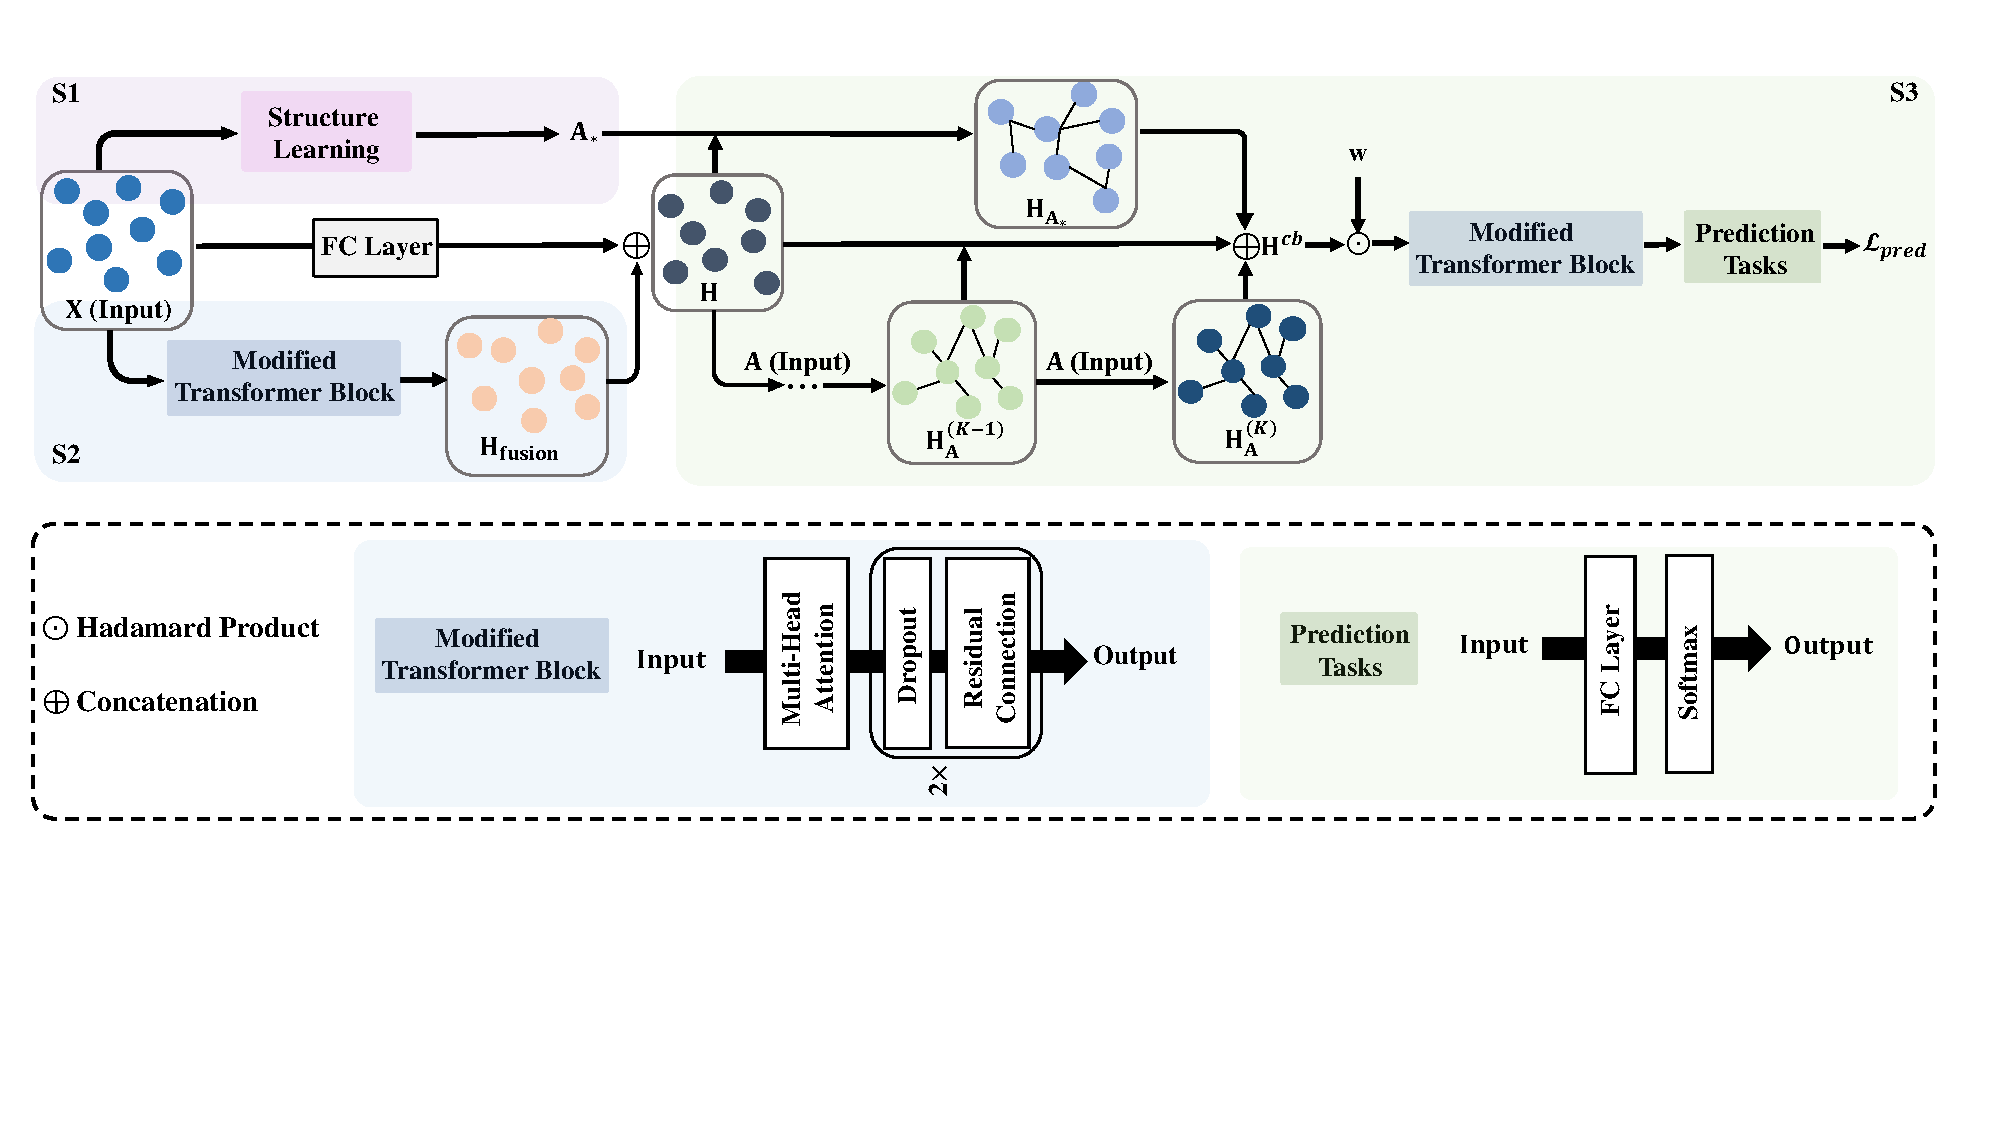
\includegraphics[page=1, width=\linewidth]{src/flowchart.pdf}
  \label{fig:flowchart}
  \caption{\textsc{GCN-SA} architecture
  \citep{jiang2024self}.}
\end{figure}

% \subsubsection{Reconnected Adjacency Matrix}

The motivation for learning a reconnected adjacency matrix
is to represent long-range connections between nodes.
An attention score matrix 
$ \mathbf{S} \in \mathbb{R}^{n\times n}$
is formed to generate a sparse reconnected adjacency matrix
$ \mathbf{A}^* \in \mathbb{R}^{n\times n}$
via $ H $-headed multi-head self-attention (MHSA):
\begin{flalign}
  \mathbf{S}
  &= \frac{1}{H} \sum_{h=1}^{H}
  \textrm{cosine}(\mathbf{X}\mathbf{W}_h^{Q}),
\end{flalign}

where $ \mathbf{W}_h^{Q} \in \mathbb{R}^{d\times p}  $
are learnable parameters corresponding to head
$ h = 1, \cdots, H $,
$ \textrm{cosine}\colon 
\mathbb{R}^{n \times p} \to [-1, 1]^{n \times n} $ 
the pairwise cosine similarity function for matrix
columns,
and $ \mathbf{S} \in [-1, 1]^{n \times n} $ the attention score matrix.
Once $ \mathbf{S} $ is obtained,
we construct the reconnected adjacency matrix
$ \mathbf{A}^* \in \left\{ 0, 1 \right\}^{n\times n} $
with a combined
$ k $NN and minimum-threshold approach:
\begin{flalign*}
  A^*_{ij} = \mathbbm{1} \left\{ 
    S_{ij} > \varepsilon \text{ or } S_{ij} \in R_i
  \right\}
\end{flalign*}

for hyperparameters $ \varepsilon, r $
and $ R_i $ denotes the $ r $ largest elements
of row $ S_{i\cdot} $.
A minor point is afterwards we set 
$ A^*_{ij} = \max \left\{ A^*_{ij}, A^*_{ji} \right\}$
to enforce symmetry.
The intention of this procedure 
is to ensure $ \mathbf{A}^* $ is \emph{sparse}
for better downstream performance \citep{jiang2024self}.
More specifically, each node attends to
$ \mathcal{O}(1) $ other nodes.
We touch on this in subsection 2.4.
For simplicity the authors denote
\begin{flalign*}
  \mathbf{A}^*
  &= \textrm{StructureLearning}(\mathbf{X}; \mathbf{W}^Q).
\end{flalign*}

parameterized by 
query parameters 
$ \mathbf{W}^Q = (
  \mathbf{W}^Q_1,
  \cdots, 
  \mathbf{W}^Q_H
) $.
Once $ \mathbf{A}^* $ is computed,
it is used downstream to compute
$ \mathbf{H}_{\mathbf{A}^*} $, 
representing aggregated long-range information:
\begin{flalign*}
  \mathbf{H}_{\mathbf{A}^{*}}
  = \mathbf{D}_*^{- \frac{1}{2}}
    \mathbf{A}^{*}
    \mathbf{D}_*^{- \frac{1}{2}}
    \mathbf{H}
\end{flalign*}

for $ \mathbf{D}_* = \text{diag}(\mathbf{A}^* \mathbf{1}_n) $ 
the degree matrix of $ \mathbf{A}^* $
and $ \mathbf{H} \in \mathbb{R}^{n \times q} $
representing node embeddings with hidden dimension $ q $.
% \mathbf{H}_\mathbf{A}^{*} 
% = \textrm{Fuse}(\mathbf{A}^{*}, \mathbf{H})
% \in \mathbb{R}^{n\times d}
% $. 
% Details on Fuse are included in the appendix.

% \subsubsection{Modified Transformer Block}

% Stages 2 and 3 of \textsc{GCN-SA} utilize a 
% transformer block:
% a fully-connected layer 
% followed by a self-attention layer.
% To mitigate overfitting
% (an issue prone to GCNs \citep{jiang2024self}),
% self-attention is followed by residual connection and dropout.
% The query parameters $ \mathbf{W}^Q $ are re-used
% in the transformer.
% We denote
% \begin{flalign*}
%   \mathbf{H} = \textrm{ModifiedTransformerBlock}(
%     \mathbf{X};
%     \mathbf{W}^Q,
%     \mathbf{W}^K,
%     \mathbf{W}^V,
%     \mathbf{W}^0
% )
% \end{flalign*}

% parameterized by the query, key, value,
% and fully-connected parameters.
% More detailed mathematical description
% can be seen is the appendix.

% \subsubsection{Feature Aggregation}

% Stepping back a little,
% GCN-SA utilize the reconnected adjacency
% matrix and the modified transformer blocks
% for feature aggregation in the following
% key sections of computation:
% \begin{enumerate}
%   \item Reconnected matrix formed from node features:
%     $ \mathbf{A}^* = \textrm{StructureLearning}(\mathbf{X}) $,
%   \item Feature embeddings 
%     $ \mathbf{H} \in \mathbb{R}^{n \times q} $ are formed 
%     from transformer block:
%     $ \mathbf{H} 
%     = \textrm{ModifiedTransformerBlock}(\mathbf{X}) $
%   \item $ \mathbf{H}_\mathbf{A}^{(k-1)},
%     \mathbf{H}_\mathbf{A}^{(k)} \in \mathbb{R}^{n \times q}$,
%     representing short-range structural information of $ G $,
%     are computed as:
%     $ \mathbf{H}_\mathbf{A}^{(k)} 
%     = \textrm{Fuse}(\mathbf{A}, \mathbf{H}_\mathbf{A}^{(k)}) $
%     for hyperparameter $ k $
%     and feature fusion function $ \textrm{Fuse} $.
%     Details on Fuse are included in the appendix.
%   \item $ \mathbf{H}^{cb} $, representing the combined information
%     of node features, short-range, and long-range structural
%     information,
%     is formed by concatenation:
%     \begin{flalign*}
%       \mathbf{H}^{cb} = \begin{bmatrix}
%         \mathbf{H}_\mathbf{A}^{(k-1)} &  
%         \mathbf{H}_\mathbf{A}^{(k)} &
%         \mathbf{H}_\mathbf{A}^{*} &
%         \mathbf{H}
%       \end{bmatrix}
%       \in \mathbb{R}^{n \times 4q}.
%     \end{flalign*}
% \end{enumerate}


\subsection{Modifying GCN-SA with Sparse SA}
This section describes the central contribution of the paper:
replacing the expensive SA computations in \textsc{GCN-SA}
with sparse equivalents.

Observe that the runtime of 
$ \text{StructureLearning}$ 
is $ \mathcal{O}(n^2d) $ due to the full SA mechanism.
We can reduce the runtime from quadratic (in $ n $)
to linear by replacing $ \text{StructureLearning} $
with a sparse SA mechanism.

\text{StructureLearning} will have 
better runtime complexity.
For instance,
\textsc{Exphormer}'s
expander attention and global attention
yield a runtime of 
$\mathcal{O}(nd)$
(we exclude \textsc{Exphormer}'s local attention
as we are only concerned with long-range dependencies).

Downstream in the model, $ \mathbf{A}^* $
is only used once more to compute $ \mathbf{H}_{A^*} $
As $ \mathbf{A}^* $ computed with the full SA
and $ k $NN + minimum-threshold approach is sparse
($\mathcal{O}(1)$ non-zero entries per row),
the computation of $ \mathbf{H}_{A^*} $
already occurs in $ \mathcal{O}(nq) $
and remains unchanged with our modified architecture.



\section{Experiments}
The purpose of this section is to evaluate the empirical
performance and runtime of 2 baseline models
(\textsc{GCN}, \textsc{GCN-SA})
and 2 \textsc{GCN-SA}-based architectures modified
with sparse SA mechanisms 
(\textsc{BigBird}, and \textsc{Exphormer})
to determine whether \textsc{GCN-SA} fitted with sparse SA
mechanisms maintain similar classification performance
whilst reducing runtime.
We present results on $ 8 $ graph datasets of varying
degrees of homophily.
More specifically, we are interested in 2 main quantities:
\begin{enumerate}
  \item Classification accuracy for each model
    evaluated on a $ 60/20/20 $ train/validation/test
    split for each dataset.
  \item Empirical runtime measurements for each model
    and each dataset on 500 epochs.
\end{enumerate}

\subsection{Models and Baselines}
We introduce
\textsc{BigBird} and \textsc{Exphormer} to
\textsc{GCN-SA}'s architecture:

\begin{itemize}
  \item \textsc{GCN-SA+Exphormer}: introduce
  \textsc{Exphormer}'s sparse SA patterns to \textsc{GCN-SA} per subsection 2.4.
  For this experiment we use default hyperparameters:
  $ 5 $-degree expander graphs,
  \texttt{Random-d} expander algorithm,
  and 1 virtual global node.
  \item \textsc{GCN-SA+BigBird}: Employ 
  \textsc{BigBird}'s 
  sparse attention mechanism to \textsc{GCN-SA} per subsection 2.4.
  Again we employ default settings.
\end{itemize}

We compare 2 modified GCN-SA with
sparse SA mechanisms to 2 baselines:
\begin{itemize}
  \item GCN: The graph convolutional nework is the base
  to our modified models. Predictions are made by
  averaging over short-range neighbouring nodes.
  \item GCN-SA: The base model of our sparse SA mechanisms
    as described in subsection 2.3.
\end{itemize}

% The GCN is introduced in
% Subsection 2.2. GCN makes predictions by aggregating local information.
% - GCN
% - GCN-SA
% - GCN-SA + bigbird
% - GCN-SA + exphormer

All parameters and hyperparameters pertaining to \textsc{GCN-SA} 
will be identical across models,
allowing fair testing to clearly 
visualize the discrepancies in results.

% To replace \textsc{GCN-SA}'s
% \textsc{StructureLearning} to 
% \textsc{SparseStructureLearning}:
% $\mathbb{R}^{n \times n} \to
% \mathbb{R}^{n \times d} $,
% we implement Principal Component Analysis (PCA)
% on input features, only retaining required information
% while reducing features size. 

% - Explain really quickly about the datasets we will be using
% - Explain for hyperparameters, we will be using the same as 
%   GCN-SA
% - Random seed is set to 42 for all experiments
% - Number of attention heads is 4


\subsection{Results}
Table 1 illustrates the node classification
accuracy of \textsc{GCN-SA+BigBird} and \textsc{GCN-SA+Exphormer}
against the accuracy of \textsc{GCN} and \textsc{GCN-SA}.
As expected, \textsc{GCN} performs the worst
out of the $ 4 $ models. 
There are no clear implications that sparse SA mechanisms 
reduce the accuracy of \textsc{GCN-SA}.

We expected the models equipped with sparse SA mechanisms
to have reduced epoch runtime. 
However, when comparing with \textsc{GNC-SA}, 
no clear improvements are seen, expecially
some models performed worse on specific datasets like
\textsc{GCN-SA+Exphormer} on citerseer. 

Considering the accuracy of \textsc{GCN-SA}
against \textsc{GCN-SA+BigBird} and \textsc{GCN-SA+Exphormer},
limited differences are seen. On the Cora dataset,
\textsc{GCN-SA} and \textsc{GCN-SA+BigBird} performed exactly 
the same, $(90.6 \pm 0.4)$. Runtime comparisons also dictate
no discrepancies between full SA and sparse SA mechanisms
with \textsc{GCN-SA + BidBird} and \textsc{GCN-SA+Exphormer}
performing practically the same as \textsc{GCN-SA}.

\begin{table}
  \caption{Node classification accuracy}
  \label{tab:sample}
  \setlength\tabcolsep{1.5pt}
  \centering
  \begin{tabular}{l c c c c c c c c c c c }
    \toprule
    \textbf{Method/Dataset} &
    Cora & Cites. & Pubmed & Chame. & 
    Squir. & Corne. & Texas & Wiscon. \\
    \midrule
    \textsc{GCN} &
    87.5$\pm$1.2 & 78.3$\pm$2.1 & 88.2$\pm$0.4 & 60.7$\pm$2.1 &
    42.4$\pm$1.2 & 62.5$\pm$3.6 & 60.9$\pm$5.7 & 60.3$\pm$4.9 \\
    \textsc{GCN-SA} &
    90.6$\pm$0.4 & 79.2$\pm$0.5 & 91.0$\pm$0.6 & 63.8$\pm$2.0  &
    46.8$\pm$1.5 & 91.5$\pm$4.9 & 90.0$\pm$2.4 & 91.0$\pm$2.4 \\
    \textsc{GCN-SA+BBird} &
    90.6$\pm$0.4 & 79.0$\pm$0.6 & 90.8$\pm$0.6 & 64.8$\pm$1.8  &
    46.7$\pm$1.7 & 91.9$\pm$4.2 & 89.4$\pm$2.4 & 91.9$\pm$2.3 \\
    \textsc{GCN-SA+Exph} &
    90.4$\pm$0.4 & 79.0$\pm$0.6 & 91.0$\pm$0.5 & 63.9$\pm$1.9  &
    46.8$\pm$1.7 & 90.1$\pm$4.1 & 90.1$\pm$2.8 & 91.8$\pm$2.3 \\
    \bottomrule
  \end{tabular}
\end{table}

\begin{figure}
  \centering
  % The next line would normally be \includegraphics instead.
  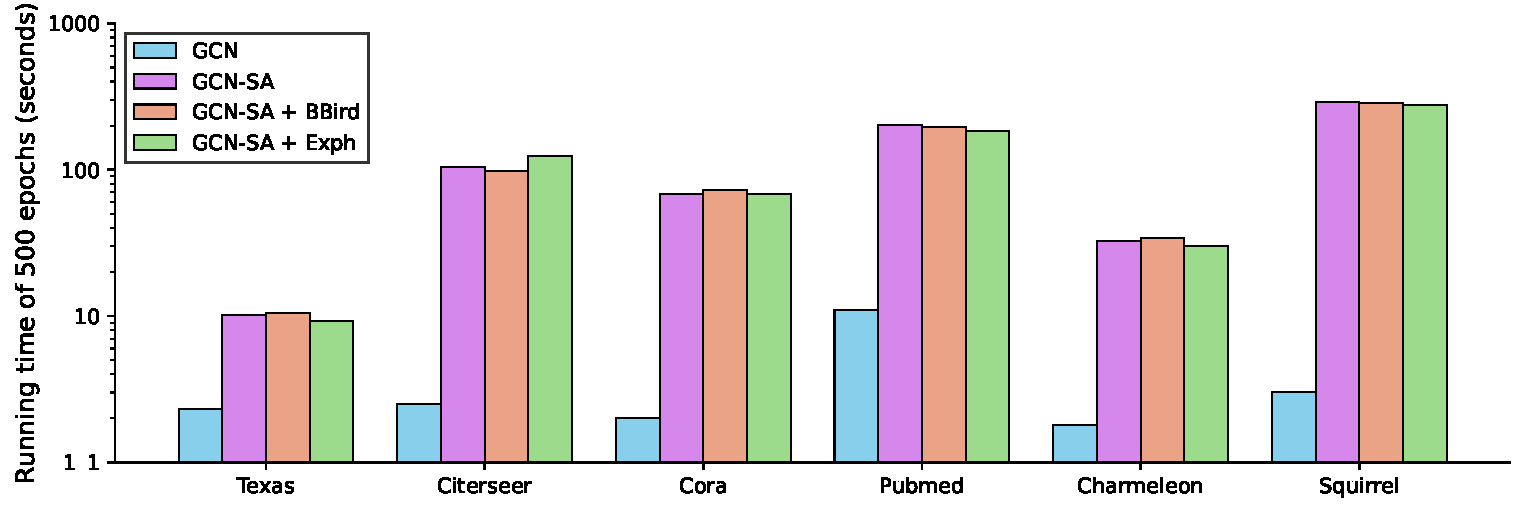
\includegraphics[page=1, width=\linewidth]{src/time_complexity.pdf}
  \caption{Runtime Comparison.}
  \label{fig:sample}
\end{figure}
% \begin{itemize}
%   \item node classification accuracy
%   \item dataset homophily ratios
%   \item model runtime for 500 epochs.
% \end{itemize}

% \begin{itemize}
%   \item Describe each experiment that you did. Say what each experiment is trying to test. 
%   \item Ideally, each experiment should only try to test one thing and you should control for as many other factors as possible. 
%   \item Subsequently, summarize the result of your experiment, in both the text and in a nice visual form such as a figure; in most cases, \textbf{a table with a huge list of numbers is not a nice way to summarize information}.
% \end{itemize}


\section{Discussion and Limitations}
Interpreting our results as-is, while we can conclude that sparse SA
mechanisms on GCN-SA preserve classification accuracy,
it cannot be said that runtime has improved dramatically.
We suspect that these results are a consequence
of limitations in our experiment design.

Graphs explored in the experiment are 
relatively small ($ < 5000 $ nodes),
mostly due to constraints in computational resources.
With more allocated time, exploration on the
Long Range Graph Benchmark datasets \citep{dwivedi2022long}
will illustrate the performance of our model for
larger low-homophily graphs, ultimately validating our models'
ability to capture low homophily for large datasets
at a substantial decrease in runtime. 
Of course this implies the need for access
to improved resources (e.g. GPUs).

% This experimentation only consider the reconnected
% adjacency matrix generation, reducing its runtime using 
% sparse SA mechanisms. GCN-SA has other transformer blocks,
% specifically a $ \text{ModifiedTransformerBlock} $, 
% utilizing multihead self attention with runtime 
% $\mathcal{O}(n^2q)$ \citep{jiang2024self}. Future exploration with
% sparse SA on this component may further reduce the runtime,
% yielding better results.

While sparse SA mechanisms like \textsc{BigBird}, 
and \textsc{Performer} introduce linear attention, they sustain 
computation overhead that dominates the per-epoch
computation time for certain graphs \citep{shirzad2023exphormer}.
In practice, better computational complexity does not
directly entail runtime improvements, as a full-attention transformer 
can be empirically faster than many sparse SA mechanisms for graphs up to 5000 nodes 
\citep{shirzad2023exphormer}. 
Again, experimentation on larger datasets may answer this concern.

Another concern is that
our exploration is limited to only one model (\textsc{GCN-SA})
due to its high performing accuracy on low homophily graphs. However,
other models with slightly worse performance (\textsc{IDGL},
\textsc{H2GCN}, \textsc{CPGNN}) \citep{jiang2024self} 
may respond better to sparse SA mechanisms. 
However it is worth noting that how SA is applied to these models
may be less clean that it is for GCN-SA.
Furthermore, additional types of sparse SA, outside 
of \textsc{Exphormer} and \textsc{BigBird} requires
investigation (e.g. \textsc{Performer}, \textsc{Longformer}).
Different SA algorithms may improve 
performance on certain models, while performing
suboptimally on others. That being said, future 
studies should consider a wider composite of SA 
mechanisms being tested on low-homophily datasets.

Finally, learning on larger graphs can 
propose ethical implications. Social media data
and other public service networks have
concerns over user privacy, as ensuring legal
consent for using individuals' data is essential.
For large datasets, it is difficult to guarantee
every individuals' consent is obtained, thus
raising issues regarding the handling of data
when consent is not explicitly given or when it is
impractical to obtain. 

% \begin{itemize}
%   \item GCN-SA has other transformer blocks,
%     this experiment was limited only to the reconnect
%     adjacency matrix generation.
%     Further exploration with sparse SA on those components
%     may further reduce the runtime.
%   \item The graphs in each of the datasets are relatively
%     small ($ < 10000 $ nodes). 
%     This doesn't reflect the performance of the models
%     on large datasets.
%     With more allotted time,
%     exploration on datasets such as 
%     the Long Range Graph Benchmark
%     \citep{dwivedi2022long}
%     will demonstrate results for larger graphs.
%   \item In practice, better computational complexity doesn't 
%     imply better empirical runtime. here's a quote to describe
%     why:
% \begin{quote}
%   While BigBird and Performer are linear attention
% mechanisms, they still incur computational overhead that
% dominates the per-epoch computation time for moderately-
% sized graphs. The GraphGPS work tackles datasets with
% graphs of up to 5,000 nodes, a regime in which the full-
% attention transformer is in fact computationally faster than
% many sparse linear-attention mechanisms. (exphormer)
% \end{quote}
%   \item 
%     Our exploration was limited only to one base model:
%     GCN-SA.
%     Despite being the highest performer,
%     other models also have close to SOTA performance.
%     We could try sparse SA on other GCNs, e.g. IDGL.
%   \item Experiment with more types of sparse SA
%     (e.g. longformer)
%   \item learning on larger graphs can be an ethical
%     problem.
%     e.g. social media data,
%     concerns over user privacy,
%     what is being done with the insights,
%     etc.
% \end{itemize}


\section{Conclusion}
In this study we 
explore the use of sparse SA mechanisms
with the recent breakthrough model
GCN-SA for learning low-homophily graphs.
We explore related approaches in the literature,
review relevant components of GCN-SA
and sparse SA,
and perform an experiment
on 3 modified GCN-SA model with sparse SA
against 2 baseline models
across 8 datasets.
From our results, 
we observe that
although sparse SA mechanisms maintain the classification
performance of GCN-SA,
it cannot be said that they reduce
empirical runtime.
Further exploration on larger datasets
with more configuration options is required.


% \begin{ack}
%   You can acknowledge useful discussion with other people who aren't coauthors here (or leave the section out).
Typically you'd also put funding here, acknowledgements for computing clusters, etc.


% \end{ack}

\printbibliography

\appendix

\section{Dataset Descriptions} \label{app:info}
This section will discuss the graph
datasets used, and define the homophily ratio classifier.

Of the $ 8 $ datasets used to validate the
proposed sparse SA \textsc{GCA-SA}-based models,
$ 3 $ are citation networks (Cora, Citeseer, Pubmed), 
$ 2 $ are Wikipedia
networks (Chameleon, Squirrel), 
and the last $ 3 $ are 
WebKB networks (Cornell, Texax, Wisconsin) (\cite{jiang2024self}).

The nodes in the citation graphs correspond to papers, each
containing an academic topic as a label. Edges are citations between
papers with each node. These datasets have a significant amount of 
does due to the amount of publications, and with certain paper
having hundreds of thousands of citations of them, the number 
of edges are seamingly large as well.

Nodes in the Wikipedia graphs are Wikipedia pages,
and edges refer to reciprocal links between pages. 
The interconnectedness of these graphs are extremely 
large because of the links between each type of squirrel
and chameleon.  

Finally, the WebKB datasets were collected
from each universitys' respective computer science
department. Nodes represent web pages and edges
are hyperlinks between web pages. These have the lowest
number of nodes as the webpages are relatively small
compared to Pubmed or Wikipedia. Here is a summary of all
the datasets from (\cite{jiang2024self}):


\begin{table}
  \caption{Summary of the datasets utilized in our experiment.}
  \label{tab:sample}
  \centering
  \begin{tabular}{lllllllll}
    \toprule
    \textbf{Datasets} &
    Cora & Citese. & Pubmed & Chamele. & 
    Squirr. & Cornell. & Texas & Wiscon. \\
    \midrule
    \textsc{Hom.ratio \textit{h}} &
    0.81 & 0.74 & 0.8 & 0.23 &
    0.22 & 0.3 & 0.11 & 0.21 \\
    \textsc{\# Nodes} &
    2708 & 3327 & 19717 & 2277 &
    5201 & 183 & 183 & 251 \\
    \textsc{\# Edges} &
    5429 & 4732 & 44338 & 31421 &
    198493 & 295 & 309 & 499 \\
    \bottomrule
  \end{tabular}
\end{table}

Based on the definition of the homophily ratio, citation networks
have the highest degree of homophily while 
Wikipedia and WebKB networks display low homophily. 
In the experimentation, we wish to preserve the predictive
accuracy of the low homophily networks while improving
the runtime through sparse SA mechanisms. 



\end{document}
